% 2015-05-21 - Emerson Ribeiro de Mello - mello@ifsc.edu.br
% \documentclass[handout,xcolor=pdftex,dvipsnames,table]{beamer}
\documentclass{beamer}

\usepackage[utf8]{inputenc}
\usepackage[T1]{fontenc}
\usepackage[english,brazil]{babel}
\let\sup\textsuperscript
\let\subs\textsubscript
% \setbeameroption{show notes on second screen=right}


% usando tema personalizado. 
% arquivo beamerthemeIFSC.sty deve estar no mesmo diretório do .tex
\usepackage{beamerthemeIFSC}


\hypersetup{pdfstartview={Fit},pdftitle={\@title},
 	pdfsubject={Engenharia de Telecomunicacoes - IFSC},pdfauthor={\@author}
}


%%%%%%%%%%%%%%%%%%%%%%%%%%%%%%%%%%%%%%%%%%%%

\newcommand{\DAY}{\the\day}
\newcommand{\MONTH}{%
    \ifcase\the\month
    \or Janeiro%
    \or Fevereiro%
    \or Março%
    \or Abril%
    \or Maio%
    \or Junho%
    \or Julho%
    \or Agosto%
    \or Setembro%
    \or Outubro%
    \or Novembro%
    \or Dezembro%
    \fi}
\newcommand{\YEAR}{\the\year}

\title{\LARGE Flip-Flops}
\author{João Cláudio Elsen Barcellos}
\date{\scriptsize \DAY~de \MONTH~de \YEAR}
\institute{Engenheiro Eletricista\\
Formado na Universidade Federal de Santa Catarina\\
campus Florianópolis\\
\url{joaoclaudiobarcellos@gmail.com}}



%%%%%%%%%%%%%%%%%%%%%%%%%%%%%%%%%%%%%%%%%%%%
\begin{document}

\captionsetup{labelformat=empty}

\begin{frame}[t]
    \maketitle
    \begin{flushleft}
        \textit{\tiny $^{*}$Créditos ao Prof. Emerson Ribeiro de Mello, o qual criou e disponibilizou o template aqui usado, via ShareLaTeX}
    \end{flushleft}
\end{frame}

\begin{frame}[t]{Plano de aula}
    \tableofcontents
\end{frame}

\def\sectionname{}
\def\insertsectionnumber{}
\def\subsectionname{}
\def\insertsubsectionnumber{}

\AtBeginSection{\frame{\sectionpage}\addtocounter{framenumber}{-1}}
\AtBeginSubsection{\frame{\subsectionpage}\addtocounter{framenumber}{-1} }
\AtBeginSubsubsection{\frame{\subsubsectionpage}\addtocounter{framenumber}{-1} }

%%%%%%%%%%%%%%%%%%%%%%%%%%%%%%%%%%%%%%%%%%%%
% Inicio do documento
%%%%%%%%%%%%%%%%%%%%%%%%%%%%%%%%%%%%%%%%%%%%

\section{Introdução}


% Slide 2: Circuitos Sequenciais (com foco em flip-flops)
\begin{frame}
    \frametitle{\insertsection}
    \begin{columns}
        \scriptsize

        \begin{column}[t]{0.38\textwidth}
            \begin{itemize}\scriptsize
                \item Circuitos nos quais a saída depende do estado atual das entradas e também de valores passados são chamados de: \textbf{circuitos sequenciais};
                \item Possuem \textbf{memória}, permitindo armazenar estados anteriores;
                \item O \textbf{flip-flop} é o elemento básico de memória: um circuito bistável que armazena 1 bit;
                \item Flip-flops são usados em: contadores, registradores, máquinas de estados, buffers e memórias digitais.
            \end{itemize}
        \end{column}
        
        \begin{column}[t]{0.58\textwidth}
            \begin{figure}
                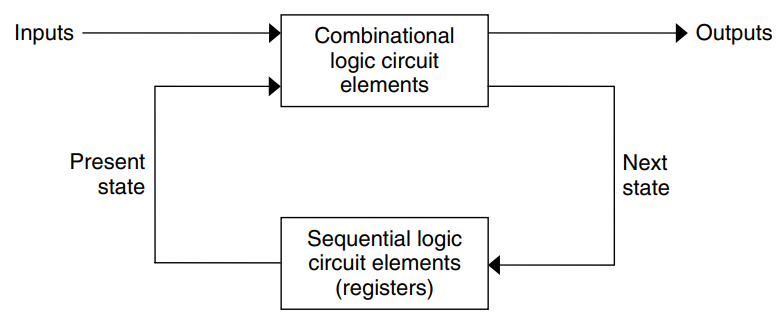
\includegraphics[width=\columnwidth]{figures/sequential_circuit.png}
                \caption*{\tiny Fonte: GROUT (2008, p. 278).}
            \end{figure}
        \end{column}   
        
    \end{columns}
\end{frame}

\section{Flip-Flops}

\begin{frame}
    \frametitle{\insertsection}
    \scriptsize
    \begin{itemize}
        \item Flip-Flops são elementos fundamentais em circuitos sequenciais, responsáveis por armazenar um bit de informação de forma estável;
        \item Diferentemente dos latches, os flip-flops são acionados por bordas de clock (subida ou descida), o que garante maior controle temporal;
        \item Funcionam como circuitos biestáveis, podendo manter seus estados indefinidamente até a chegada de um novo pulso de controle;
        \item São utilizados na construção de registradores, contadores e máquinas de estados, sendo blocos essenciais na lógica sequencial síncrona.
    \end{itemize}
\end{frame}

\begin{frame}
    \frametitle{\insertsection}
    \scriptsize
    \begin{itemize}
        \item Flip-Flops também são usados para armazenar um único bit de informação;
        \item E também pode ser classificado como um circuito biestável, já que possui dois estados estáveis: 0 ou 1;
        \item No entanto, os Flip-Flops são formados por latches;
        \item Dessa forma são elementos de memória mais ``complexos''.
    \end{itemize}
\end{frame}

\subsection{Flip-Flop SR}

\begin{frame}
    \frametitle{\insertsubsection}
    \scriptsize
    \begin{itemize}
        \item O Flip-Flop SR (Set-Reset) é um circuito sequencial básico usado para armazenamento de um bit de informação;
        \item Sua operação é controlada por um sinal de clock, que define o momento em que as entradas são amostradas;
        \item Quando o clock apresenta uma borda de subida (↑), o estado do Flip-Flop pode ser alterado conforme os sinais de entrada S e R;
        \item A combinação S = R = 1 é considerada inválida, pois leva a uma condição indefinida na saída.
    \end{itemize}

    \vspace{0.5em}
    \centering
    \captionof{table}{Tabela Verdade - Flip-Flop SR com Clock}
    \begin{tabular}{|c|c|c|c|c|}
        \hline
        CLK & S & R & Q(t) & Q(t+1) \\
        \hline
        ↑ & 0 & 0 & Q     & Q \\
        ↑ & 0 & 1 & Q     & 0 \\
        ↑ & 1 & 0 & Q     & 1 \\
        ↑ & 1 & 1 & Q     & Indef. \\
        \hline
    \end{tabular}
  
\end{frame}

\subsection{Flip-Flop D}

\begin{frame}
    \frametitle{\insertsubsection}
    \scriptsize
    \begin{columns}
        % Coluna com texto e tabela
        \begin{column}[t]{0.5\textwidth}
            \begin{itemize}
                \item O Flip-Flop D (Data ou Delay) armazena o valor da entrada D na borda de subida do clock;
                \item Garante que a saída Q siga D apenas no momento apropriado, evitando condições indesejadas;
                \item Muito utilizado em registradores e sistemas de armazenamento temporário.
            \end{itemize}

            \vspace{0.5em}
            \centering
            \captionof{table}{Tabela Verdade - Flip-Flop D com Clock}
            \begin{tabular}{|c|c|c|c|}
                \hline
                CLK & D & Q(t) & Q(t+1) \\
                \hline
                ↑ & 0 & Q & 0 \\
                ↑ & 1 & Q & 1 \\
                \hline
            \end{tabular}
            \caption*{\tiny Fonte: Adaptado de HARRIS; HARRIS (2015)}
        \end{column}

        % Coluna com a imagem (diagrama de tempo)
        \begin{column}[t]{0.45\textwidth}
            \centering
            \captionof{figure}{}
            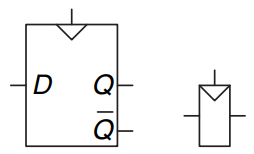
\includegraphics[width=\columnwidth]{figures/flipflop_d_symbols.png}
            
        \end{column}
    \end{columns}
\end{frame}
 \begin{frame}
\frametitle{Aplicação Flip-flop D}
\begin{figure}
    \centering
    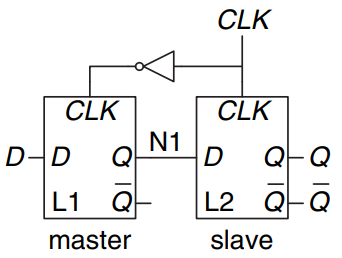
\includegraphics[width=0.6\columnwidth]{figures/flipflop_d_schematic.png}
    \caption{Aplicação Flip-flop D.}
\end{figure}
\end{frame}


\subsection{Flip-Flop JK}
% Slide - Flip-Flop JK
\begin{frame}
\frametitle{Flip-Flop JK}
\begin{itemize}
    \item O Flip-Flop JK é uma modificação do Flip-Flop SR que elimina a condição indesejada.
    \item Quando J = K = 1, o estado do Flip-Flop é invertido (toggle).
    \item As mudanças de estado ocorrem na borda de subida do clock.
    \item Tabela verdade:
\end{itemize}

\begin{table}[]
\centering
\begin{tabular}{|c|c|c|c|c|}
\hline
CLK & J & K & Q(t) & Q(t+1) \\
\hline
↑   & 0 & 0 & Q     & Q \\
↑   & 0 & 1 & Q     & 0 \\
↑   & 1 & 0 & Q     & 1 \\
↑   & 1 & 1 & Q     & $\overline{Q}$ \\
\hline
-   & X & X & Q     & Q \\
\hline
\end{tabular}
\end{table}
\end{frame}


% Slide - Flip-Flop T

\subsection{Flip-Flop T}

\begin{frame}
    \frametitle{Flip-Flop T}
    \begin{itemize}
        \item O Flip-Flop T (Toggle) inverte o estado de saída a cada transição de clock quando T = 1.
        \item É uma simplificação do Flip-Flop JK, onde J = K.
        \item Tabela verdade com clock na borda de subida:
    \end{itemize}

    \vspace{0.5em}
    \centering
    \begin{tabular}{|c|c|c|c|}
        \hline
        CLK & T & Q(t) & Q(t+1) \\
        \hline
        ↑ & 0 & Q & Q \\
        ↑ & 1 & Q & $\overline{Q}$ \\
        \hline
    \end{tabular}
\end{frame}

\section{Aplicações dos Flip-Flops}
% Slide - Aplicações dos Flip-Flops
\begin{frame}
\frametitle{Aplicações dos Flip-Flops}
\begin{itemize}
    \item Registradores
    \item Contadores binários
    \item Divisores de frequência
    \item Armazenamento de dados temporários
    \item Máquinas de estados finitos
\end{itemize}
\end{frame}


\section{Conclusão}
% Slide - Conclusão
\begin{frame}
\frametitle{Conclusão}
\begin{itemize}
    \item Flip-Flops são blocos fundamentais na construção de circuitos sequenciais.
    \item Cada tipo possui características e aplicações específicas.
    \item A escolha adequada depende da lógica e da funcionalidade desejada.
\end{itemize}
\end{frame}

\section{Atividade Prática}


 \begin{frame}
\frametitle{Atividade Prática}
\begin{figure}
    \centering
    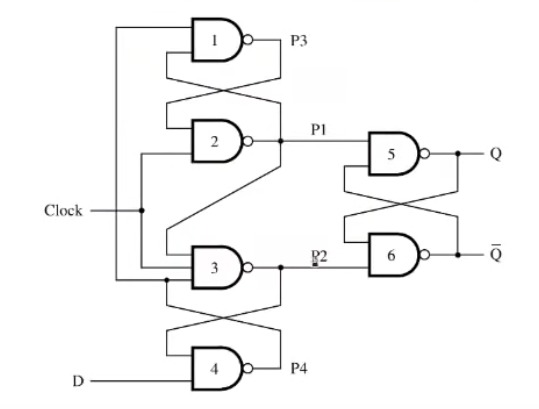
\includegraphics[width=0.7\columnwidth]{figures/Atividade_Pratica.jpeg}
    \caption{Atividade Prática.}
\end{figure}
\end{frame}

\section{Referências}
% Slide - Referências
\begin{frame}
\frametitle{Referências}
\begin{itemize}
    \item Mano, M. M., \& Ciletti, M. D. (2013). Digital Design.
    \item Tocci, R., Widmer, N., \& Moss, G. (2010). Sistemas Digitais: Princípios e Aplicações.
\end{itemize}
\end{frame}

\end{document}
